\documentclass{article}
\usepackage[utf8]{inputenc}

\title{Apostila - Microsoft Windows Movie Maker}
\author{
    Pedro Augusto Duarte de Almeida\\
    \and
    Rodrigo Maia Pereira\\
    \and
    Claudiene Aurora de Cassia Gomes\\
    \and
    Dhenerson Augusto Carneiro\\
    \and
    Patrick Sorrentino Reis\\
    \and
    Alan Fagner Nunes\\
}

\date{}

\usepackage{natbib}
\usepackage{graphicx}

\begin{document}

\maketitle

\section{Introdução:}
O Windows Movie Maker é um software (programa) de edição de vídeos da Microsoft.
Com este programa é possível que qualquer pessoa insira áudio, títulos, textos personalizados e efeitos de transição em suas fotos.

\begin{figure}[h!]
\centering
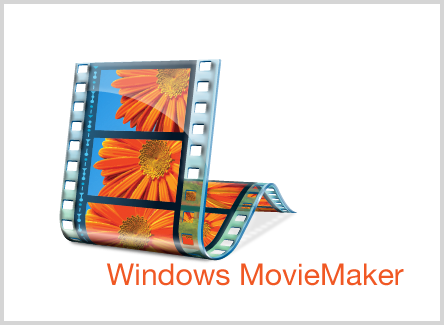
\includegraphics[scale=0.35]{movie-maker.png}
\end{figure} 

Existem vários tipos de filmes que podem ser criados no Movie Maker, e um deles pode ser feito a partir de fotos tiradas com celulares, máquinas fotográficas ou filmadoras.\\

Separe as fotos, os textos, e as músicas que pretende usar em seu filme. Uma dica importante é colocar todas as imagens imagens e músicas salvos na mesma pasta em seu computador, pois até a hora de salvar o seu projeto como filme, o Windows Movie Maker vai precisar encontrar tudo numa pasta só. Fique calmo, vamos explicar melhor ao longo do tutorial. \\

Bom, agora que você já tem todo o material para começar, vamos lá?\\

O exemplo a seguir mostra como criar um file usando todos os recursos do
Movie Maker. Aproveite!

\newpage

\section{Separando suas fotos e músicas:}
\begin{enumerate}
\item Crie no seu computador uma pasta para o seu projeto
\item Vá até a pasta Meus Vídeos
\item Clique com o botão direito e escolha a opção Novo / Pasta;
\item Escreva como nome da pasta o nome do seu filme;
\item Abra a pasta que acabou de criar e dentro dela crie outra pasta com o nome Fotos e Músicas;
\item Salve dentro desta pasta todas as imagens, vídeos e áudios que pretende usar em seu projeto
\end{enumerate}

\section{Criando um projeto:}
\begin{enumerate}
\item Clique em Arquivo / Salvar Projeto;
\item Vá até a pasta Meus Vídeos;
\item Salve na pasta que criou com o nome do projeto;
\item Pronto! Agora podemos começar!
\end{enumerate}

\begin{figure}[h!]
\centering
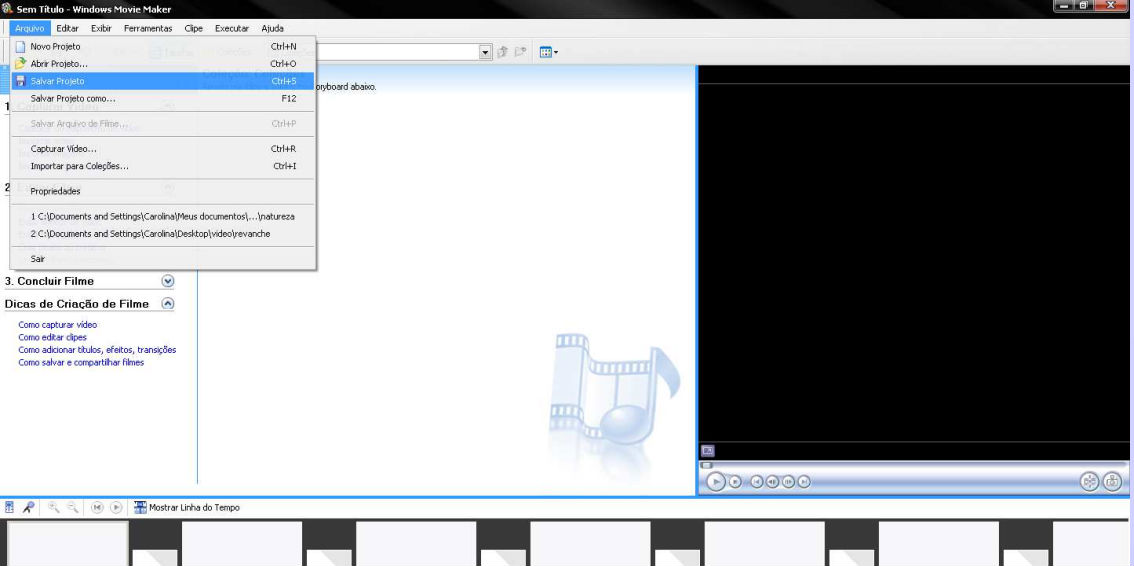
\includegraphics[scale=0.35]{segundoPasso.jpg}
\end{figure}

\newpage

\section{Importando suas fotos e músicas:}
\begin{enumerate}
\item Do lado esquerdo da tela \textbf{Captura Vídeo} , clique em \textbf{Importar Imagens}. Busque na pasta do projeto as imagens que separou e clique em \textbf{Importar}. No campo tipos de arquivo selecione \textbf{Arquivos de Imagens};
\item Faça o mesmo com os vídeos e áudios que pretende usar no filme;
\item No centro da tela você formará uma coleção com os arquivos que vai usar no projeto.
\end{enumerate}

\section{Montando o storyboard:}
\begin{enumerate}
\item Para montar o storyboard é simples: clique na imagem que deseja colocar no início do filme e arraste para o primeiro quadrado em branco na parte inferior da tela;
\item Faça o mesmo com as demais fotos e vídeos lembrando sempre da ordem que deseja que apareçam em seu projeto;
\item Se deseja ter uma idéia de como ficará, selecione a primeira imagem no storyboard e na tela ao lado clique no play.
\end{enumerate}

\section{Inserindo uma música:}
\begin{enumerate}
\item Para inserir uma música em seu filme clique em \textbf{Mostrar Linha do Tempo} na parte inferior da tela;
\item A música que você quer colocar deverá estar em sua coleção. Clique e arraste o arquivo da música para a segunda parte da linha do tempo;
\item Para que a música comece junto com o filme, posicione no início da linha.
\end{enumerate}

\section{Inserindo textos:}
\begin{enumerate}
\item Para inserir textos em seu filme use o menu \textbf{Editar Filme} que fica do lado esquerdo da tela. Para isso, clique em \textbf{Criar Títulos ou Créditos};
\item Clique em \textbf{Adicionar Título};
\item Digite o título no campo de texto, para formatar clique em \textbf{Alterar fonte e a cor do texto};
\item Para escolher a forma como o texto vai aparecer clique em \textbf{Alterar a animação do título};
\item Para finalizar, clique em \textbf{Concluir}.
\end{enumerate}

\newpage

\section{Inserindo efeitos especiais:}
\begin{enumerate}
\item Para inserir um efeito, ou vários, em seu filme, clique no menu lateral \textbf{Editar filme} em \textbf{Exibir efeitos de vídeo}. Os efeitos devem aparecer no centro da tela, onde antes era vista a nossa coleção de imagens, vídeos e áudio;
\item Escolha o efeito que mais combina com o seu filme, clique nele e arraste até o storyboard, dentro do quadrado com uma estrela dentro, no canto inferior
esquerdo; Pronto! Solte o efeito e aperte o play para visualizar;
\item Faça isso em todas as imagens e vídeos do storyboard. 
\item \textbf{Dica:} Você pode escolher um efeito diferente para cada quadrado!
\end{enumerate}

\section{Inserindo animações de transições:}
\begin{enumerate}
\item Para inserir um efeito, ou vários, em seu filme, clique no menu lateral \textbf{Editar filme} em \textbf{Exibir transições de vídeo}; As opções devem aparecer no centro da tela, onde antes eram vistos os efeitos de vídeo;
\item Escolha a transição que mais combina com o seu filme, clique nele e arraste até o storyboard, dentro do quadrado pequeno que fica entre cada imagem;
Pronto! Solte o efeito e aperte o play para visualizar.
\item \textbf{Dica:} Você pode escolher uma transição diferente para cada quadrado.
\end{enumerate}

\section{Fazendo a edição final:}
\begin{enumerate}
\item Chegou a hora de ver se o tempo de cada imagem, junto com a música e os efeitos estão de acordo com o planejado;
\item Na parte inferior da tela clique em \textbf{Mostrar Linha do Tempo};
\item Repare que na parte superior da linha do tempo existe uma régua que mostra o tempo. Cada imagem inserida no filme aparece na ordem escolhida. Se deseja diminuir o tempo de cada imagem, clique nela e com a seta vermelha arraste para a esquerda (para diminuir seu tempo) ou para direita (para aumentar o tempo);
\item Faça o mesmo na segunda linha para ajustar o tempo da música. Pronto! Vamos salvar o projeto como filme?
\end{enumerate}


\end{document}